%%%%% Document Setup %%%%%%%%

\documentclass[10pt,twocolumn]{revtex4-2}    % Font size (10,11 or 12pt) and column number (one or two).

\AtBeginDocument{
  \abovedisplayskip=6pt plus 2pt minus 2pt
  \belowdisplayskip=6pt plus 2pt minus 2pt
  \abovedisplayshortskip=2pt plus 1pt
  \belowdisplayshortskip=4pt plus 2pt minus 2pt
}

\makeatletter
\renewcommand{\subsection}{\@startsection{subsection}{2}{\z@}%
  {-2.5ex plus -0.5ex minus -0.2ex}%  % space before (negative = no indent after)
  {2.5ex plus 0.2ex}%                  % space after
  {\normalfont\normalsize\bfseries}}
\makeatother

\usepackage{lipsum}
\usepackage{times}                          % Times New Roman font type

\usepackage[a4paper, left=1.85cm, right=1.85cm,top=1.85cm, bottom=1.85cm]{geometry}       % Defines paper size and margin length

\usepackage[font=small, labelfont=bf]{caption}                      % Defines caption font size as 9pt and caption title bolded

\hyphenpenalty=10000
\exhyphenpenalty=10000

\usepackage[ruled,vlined,linesnumbered]{algorithm2e}

\usepackage{optidef}

\usepackage{booktabs}                       % For table
\setlength{\tabcolsep}{20pt}  

\usepackage{tikz}                           % For drawing figures
\usetikzlibrary{arrows.meta, decorations.markings, calc}

\usepackage{parskip}                        % Adds space between paragraphs and removes indentation
%\setlength{\parskip}{0.5ex plus 0.2ex minus 0.1ex}

\usepackage{subcaption}                     % For sensitivities in results section

\usepackage{graphics,graphicx,epsfig,ulem}	% Makes sure all graphics works
\usepackage{amsmath} 						% Adds mathematical features for equations

\usepackage{etoolbox}                       % Customise date to preferred format

\makeatletter
\patchcmd{\frontmatter@RRAP@format}{(}{}{}{}
\patchcmd{\frontmatter@RRAP@format}{)}{}{}{}
\renewcommand\Dated@name{}
\makeatother

\usepackage{fancyhdr}


\pagestyle{fancy}                           % Insert header
\renewcommand{\headrulewidth}{0pt}
\lhead{S. Coulthurst}                          % Your name
\rhead{Minimum Fuel Transfer Trajectory Between Earth and Moon in the Circular Restricted Three Body Problem}            % Your report title               

\def\bibsection{\section*{References}}        % Position reference section correctly


%%%%% Document %%%%%
%\setcitestyle{authoryear,round}    
\begin{document}


\title{Minimum Fuel Transfer Trajectory Between Earth and Moon in the Planar Circular Restricted Three Body Problem} 
\date{Submitted: \today{}}
\author{Samuel James Coulthurst}
\affiliation{\normalfont L3 Computing Project, Group C4}


\begin{abstract}              

This investigation aimed to find a bi-impulsive transfer trajectory in the planar circular restricted three body problem from a low Earth orbit of altitude 167~km to a low Lunar orbit of altitude 100~km using less fuel than a Hohmann transfer. The problem was formulated as a non-linear programming problem and solved using a hierarchical grid search. The value obtained for the total change in velocity required was $\Delta v_{total} = 3.958 ~\mathrm{km/s}$, which is 0.09\% higher than the Hohmann transfer value of $\Delta v_{total} = 3.954~\mathrm{km/s}$. The optimal trajectory found does not save fuel over the Hohmann transfer. The search did not extend to sufficiently long times of flight to find a low energy transfer due to the time complexity of the grid search algorithm. 

\end{abstract}

\maketitle

\thispagestyle{plain} % produces page number for front page

\section{Introduction} 

Humans have not walked on the surface of the Moon since 1972. However, in the past decade, there has been increased interest from multiple space agencies and private companies in exploring far beyond Earth's orbit. In particular, the Moon is considered the cornerstone of near future space exploration, with NASA and SpaceX aiming to send manned missions to the Moon in 2026 \cite{ESA_ref_cornerstone, nasa_artemis}. 

\vspace{0.5em}

In order to send human and robotic missions to the Moon efficiently, it is crucial to find optimal trajectories that minimize fuel consumption. The cost of launching payload to low Earth orbit (LEO) for the SpaceX Falcon 9 is approximately $\$2{,}940 \, \text{kg}^{-1}$, highlighting the enormous financial incentive to reduce propellant mass \cite{jones2023}. 

\vspace{0.5em}

In 1903, Russian rocket scientist Tsiolkovsky discovered that the change in mass of a rocket, due to fuel usage or otherwise, is directly related to the change in velocity of the rocket. This is shown below in Eq. \ref{Eq:RocketEquation} which is known as the Rocket Equation \cite{tsiolkovsky1903}.

\begin{equation}
    \Delta v = v_{e} ln(\frac{m_{0}}{m_{f}}),
    \label{Eq:RocketEquation}
\end{equation}
\vspace{0.5em}

where $\Delta v$ is the impulsive change in the spacecraft's velocity and $v_{e}$ is the effective exhaust velocity. $m_{0}$ and $m_{f}$ are the masses of the rocket before and after the change in velocity has occurred respectively. Hence, minimising the fuel used for a transfer is equivalent to minimising the sums of the $\Delta v$'s for all manoeuvres involved. For a typical chemical rocket, propellant can account for up to 90\% of the total launch mass, meaning that even small reductions in the required $\Delta v_{total}$ can yield substantial savings in cost and mass \cite{nasa_rocket_equation}.

\vspace{0.5em}

The Earth-Moon transfer has been extensively studied by many researchers. In particular, the transfers from low Earth orbit (LEO) of height 167~km to low lunar orbit (LLO) of 100~km have frequently been investigated. The simplest and fastest approach, but not the most fuel efficient, is the Hohmann transfer. Discovered in 1925, the Hohmann transfer uses a two body approximation and consists of two impulsive burns \cite{Hohmann1925}. The $\Delta v_{total}$ of the manoeuvres required has a value of $3.954~\mathrm{km/s}$ \cite{Qi_Xu_2016}. It is a common benchmark value for transfer techniques. Another method under the two body approximation is the patched-conics transfer. By carefully switching the sphere of influence along the trajectory, the rocket's motion is only governed by either the Earth or the Moon at a given time. These two "classical" transfers were used for all lunar missions from the 1960s to the 1980s, including the Apollo missions. The $\Delta v_{total}$ required for Apollo 11 to be in orbit around the Moon was $\Delta v_{total} = 4.136~\mathrm{km/s}$ \cite{Riche1969}.

\vspace{0.5em}

To reduce this total cost, the low energy transfer (LET) was put forward. Belbruno proposed the Weak Stability Boundary (WSB) theory to achieve lunar capture with minimal $\Delta v_{total}$ using invariant manifolds \cite{Belbruno1993}. Together with Miller, they numerically demonstrated that the $\Delta v_{total}$ needed for the transfer was 18\% less than that of the Hohmann transfer with a time of flight, $T$, of 3-5 months. Belbruno's WSB transfer was successfully demonstrated by the Japanese spacecraft Hiten, which arrived in orbit around the Moon on October 2, 1991. More recently, NASA's GRAIL mission in 2011 exploited similar concepts to reach the Moon from the Earth \cite{roncoli2010}. Sweetser derived the theoretical minimum $\Delta v_{total}$ for the LEO to LLO transfer in the PCR3BP, which equals $3.726~\mathrm{km/s}$ \cite{Sweetser1991}. The corresponding time of flight for this minimum $\Delta v_{total}$ is infinite due to the asymptotic approach along invariant manifolds.

\vspace{0.5em}

Topputo further investigated the bi-impulsive Earth-Moon transfer problem using direct transcription and multiple shooting, finding thousands of solutions in a four body model \cite{topputo2013}. His results establish that the room for significant $\Delta v_{total}$ improvement over the Hohmann transfer is modest, with the Sweetser bound of $3.726~\mathrm{km/s}$ acting as a hard lower limit.  

\vspace{0.5em}

The objective of this report is to find a lower fuel transfer trajectory from LEO of 167~km to LLO of 100~km in the Planar Circular Restricted Three Body Problem (PCR3BP) than the Hohmann transfer. This will be achieved using a hierarchical grid search method. 

\clearpage

\section{Theory}
\label{sec:Theory}

In this section, the basic theories of the PCR3BP and the Hohmann transfer are introduced. Subsequently, the algorithm used for numerical integration is outlined.

\subsection{Planar Circular Restricted Three Body Problem}
\label{sec:Planar Circular Restricted 3 Body Problem}

The PCR3BP describes the motion of an object with a negligible mass under the influence of two massive bodies (primaries). In this paper, these two bodies are the Earth, with mass $m_1$, and the Moon, with mass $m_2$, both of which are assumed to be point masses in circular orbits around their barycenter. Furthermore, it is assumed all motion lies within a plane, and hence the rocket's motion can be described with two degrees of freedom.

As usual, this dynamical system is implemented in a non-dimensional coordinate system. The distance unit ($L*$) was defined as distance between $m_1$ and $m_2$ ($L* = 384,400$ km for the Earth-Moon system). The time unit ($T*$) was defined such that the mean angular motion of the primaries about the system's centre of mass was unity ($T* = 4.343$ days).

The PCR3BP in the rotating barycentric frame is depicted below in Fig. \ref{fig:cr3bp}. 

\vspace{1em}
\begin{figure}[h]
    \centering
    \begin{tikzpicture}[scale=3]
        % Axes
        \draw[->] (-1.3,0) -- (1.3,0) node[right] {$x$};
        \draw[->] (0,-0.5) -- (0,1.2) node[above] {$y$};

        % Primaries
        \filldraw[blue] (-0.3,0) circle (2pt) node[above=8pt] {$m_1$};
        \filldraw[gray] (0.7,0) circle (1.5pt) node[above right=8pt] {$m_2$};

        % Position labels
        \node[below=5pt] at (-0.3,0) {$(-\mu, 0)$};
        \node[below=5pt] at (0.7,0) {$(1-\mu, 0)$};

        % Centre of mass
        \filldraw (0,0) circle (0.5pt) node[below right] {CoM};

        % Test particle (rocket)
        \filldraw (0.5,0.8) circle (1pt) node[above right] {Rocket};

        % Distance vectors
        \draw[dashed, ->] (-0.3,0) -- (0.5,0.8) node[midway, left] {$r_1$};
        \draw[dashed, ->] (0.7,0) -- (0.5,0.8) node[midway, right] {$r_2$};
    \end{tikzpicture}
    \caption{Planar circular restricted three body problem in the rotating frame for the Earth-Moon system as viewed from the z axis.}
    \label{fig:cr3bp}
\end{figure}

Where 
\begin{equation}
    \mu = \frac{m_2}{m_1 + m_2},
\end{equation}
is the mass ratio of the system. For the Earth-Moon system, $\mu = 0.01215058$.

The Lagrangian of the system can be written as
\begin{equation}
    L = \frac{1}{2}(\dot{x}^2 + \dot{y}^2) + (x\dot{y} - y\dot{x}) + \frac{1}{2}(x^2+y^2) + \frac{1-\mu}{r_1} + \frac{\mu}{r_2},
\end{equation}

the equations of motion for the rocket are then given by:

\begin{equation}
    \ddot{x} - 2\dot{y} = \frac{\partial \Omega}{\partial x},
    \label{eq:EOM1}
\end{equation}
\begin{equation}
    \ddot{y} + 2\dot{x} = \frac{\partial \Omega}{\partial y},
    \label{eq:EOM2}
\end{equation}

where $\Omega$ is the effective potential of the system,

\begin{equation}
    \Omega(x, y) = \frac{1}{2}(x^2 + y^2) + \frac{1-\mu}{r_1} + \frac{\mu}{r_2} + \frac{1}{2}\mu(1-\mu),
\end{equation}

and $r_1$ and $r_2$ are the distances from the rocket to the Earth and Moon respectively, given by:

\begin{equation}
    r_1 = \sqrt{(x + \mu)^2 + y^2},
\end{equation}
\begin{equation}
    r_2 = \sqrt{(x - 1 + \mu)^2 + y^2}.
\end{equation}

The Lagrangian does not explicitly depend on time, hence there is a conserved quantity of the rocket's motion in the rotating frame. This is known as the Jacobi constant (or Jacobi integral) and is given by Eq. \ref{eq:JacobiIntegral}

\begin{equation}
    C = 2\Omega(x, y) - (\dot{x}^2 + \dot{y}^2).
    \label{eq:JacobiIntegral}
\end{equation}

\subsection{Hohmann Transfer}
\label{sec:Hohmann Transfer}

The Hohmann transfer is a well known orbit transfer method which could be used to transfer from the Earth to the Moon \cite{Hohmann1925}. It is the simplest type of transfer and is often used as a reference to compare values of $\Delta v_{total}$ to other transfer types. It uses a two body approximation and is bi-impulsive. The first impulse is applied to the rocket in LEO to put it on a transfer trajectory. The second impulse is applied at the end of the transfer trajectory to put the rocket into LLO. The Hohmann transfer is depicted in Fig. \ref{fig:Hohmann transfer}.


\vspace{1em}
\begin{figure}[h]
    \centering
    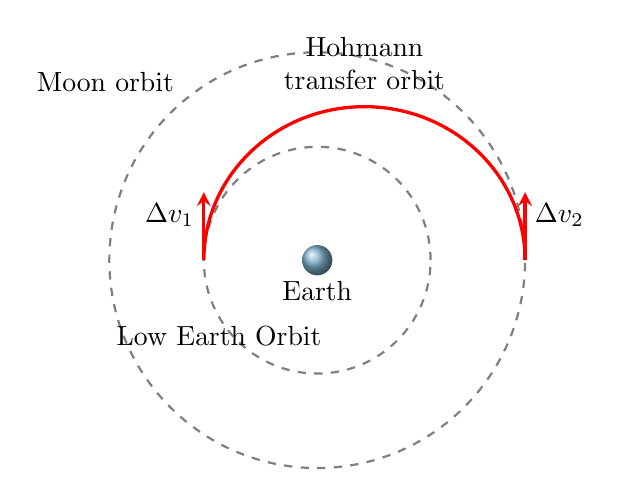
\begin{tikzpicture}[scale=0.48, every node/.style={transform shape=false}]

        % Radii
        \def\rLEO{3.0}
        \def\rMoon{5.5}

        % Hohmann ellipse parameters
        \pgfmathsetmacro{\aTransfer}{(\rLEO + \rMoon) / 2}
        \pgfmathsetmacro{\bTransfer}{sqrt(\rLEO * \rMoon)}
        \pgfmathsetmacro{\cTransfer}{\aTransfer - \rLEO}

        % LEO
        \draw[gray, thick, dashed] (0,0) circle (\rLEO);

        % Lunar Orbit
        \draw[gray, thick, dashed] (0,0) circle (\rMoon);

        % Hohmann transfer ellipse (upper half only)
        \draw[red, very thick] 
            ({-\rLEO}, 0) arc[
            x radius=\aTransfer,
            y radius=\bTransfer,
            start angle=180,
            end angle=0
            ];

        % Earth
        \shade[ball color=blue!60!green!50!white] (0,0) circle (0.4);

        % Delta-v arrows
        \draw[-stealth, red, very thick] ({-\rLEO}, 0) -- ({-\rLEO}, 1.8);
        \node[left] at ({-\rLEO}, 1.2) {$\Delta v_1$};

        \draw[-stealth, red, very thick] ({\rMoon}, 0) -- ({\rMoon}, 1.8);
        \node[right] at ({\rMoon}, 1.2) {$\Delta v_2$};

        % Labels
        \node[above left] at ({-\rMoon*cos(50)}, {\rMoon*sin(50)}) 
            {Moon orbit};

        \node[below] at ({-\rLEO*cos(30)}, {-\rLEO*sin(30)}) 
            {Low Earth Orbit};

        \node at (0, -0.8) {Earth};

        \node[above, align=center] at ({\cTransfer}, {\bTransfer + 0.2}) 
            {Hohmann\\transfer orbit};

    \end{tikzpicture}
    \caption{Hohmann transfer from low Earth orbit to low lunar orbit}
    \label{fig:Hohmann transfer}
\end{figure}

The value obtained for the total change in velocity $\Delta v_{total}$ for a Hohmann transfer from an LEO of 167~km to LLO of 100~km is $3.954 ~\mathrm{km/s}$ \cite{Qi_Xu_2016}. This is the value this report aims to improve upon. 

\subsection{Dormand-Prince Algorithm}
\label{sec:Dormand-Prince Algorithm}

The equations of motion, Eqs.~(\ref{eq:EOM1}) and~(\ref{eq:EOM2}), were 
integrated numerically using the Dormand-Prince DOP853 
algorithm~\cite{hairer1993}, an explicit 8th order Runge Kutta method 
with an adaptive step size control. The algorithm was implemented using SciPy~\cite{virtanen2020}.

DOP853 advances the solution using an 8th-order approximation and 
estimates the local truncation error by comparison with lower order 
(5th and 3rd) approximations obtained from the same function evaluations. 
These two error estimates are combined into a single scalar measure 
$\mathrm{err}$, scaled component wise by
%
\begin{equation}
    \mathrm{sc}_i = \mathrm{atol} + \mathrm{rtol} \cdot |y_i|,
    \label{eq:sc}
\end{equation}
%
where $\mathrm{atol}$ and $\mathrm{rtol}$ are the absolute and relative 
tolerances, respectively. A step is accepted when $\mathrm{err} \leq 1$; 
otherwise the step size is reduced and the step is retried. Accepted steps 
are followed by a step size update of the form $h_{\mathrm{new}} = h 
\cdot f \cdot \mathrm{err}^{-1/8}$, where $f < 1$ is a safety factor. 

\section{Method}
\label{sec:Method}

In this section, the problem will be formulated and the specific optimisation methods used to solve the problem will be described.

\subsection{Problem Formulation}

The minimum fuel transfer problem was formulated as a non-linear programming (NLP) problem. 

%\vspace{-3ex}
\begin{subequations}\label{eq:opt}
\begin{align}
  \underset{\vec{x}}{\text{minimise}} \quad & \Delta v_{\text{total}}(\vec{x}) = \Delta v_{1}(\vec{x}) + \Delta v_{2}(\vec{x}) \label{eq:opt_obj} \\
  \text{subject to} \quad & c(\vec{x}) = \lvert \vec{r}_{\text{rocket}}(\vec{x}) - \vec{r}_{\text{LLO}} \rvert = 0 \label{eq:opt_con}
\end{align}
\end{subequations}
%\vspace{-3ex}

$\Delta v_{total}(\vec{x})$ is the objective function, which is the total change in velocity required for the transfer. The constraint function $c(\vec{x})$ ensures that the rocket terminates in a closed, circular orbit at the correct altitude above the Moon.

The decision variables $\vec{x}$ are 

%\vspace{-3ex}
\begin{equation}
    \vec{x} = [\theta, \Delta v_1, \alpha, T],
\end{equation}
%\vspace{-3ex}

where $\theta$ is the angle of the initial position of the rocket in LEO, $\Delta v_1$ is the magnitude of the first impulse applied to the rocket, $\alpha$ is the angle this impulse is applied at relative to the tangential direction, and $T$ is the time of flight as shown in Fig. \ref{fig:earth-moon-transfer}.

\begin{figure}[h]
    \centering
    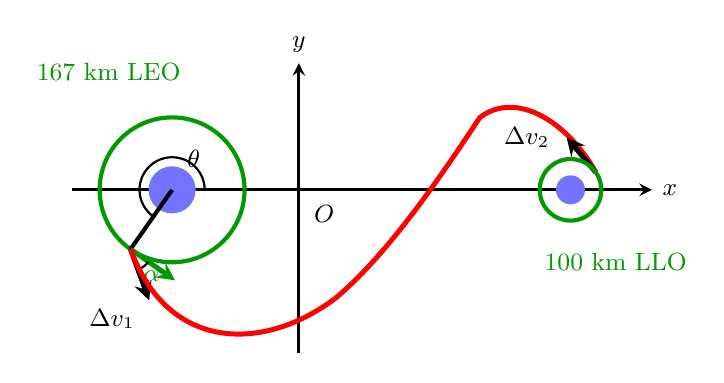
\begin{tikzpicture}[scale=0.23, every node/.style={transform shape=false}]
    
        % ---- Parameters ----
        \def\Ex{-7}        % Earth centre x
        \def\Ey{0}         % Earth centre y
        \def\Mx{15}        % Moon centre x
        \def\My{0}         % Moon centre y
        \def\rEarth{1.3}   % Earth radius (visual)
        \def\rLEO{4}       % LEO orbit radius
        \def\rMoon{0.8}    % Moon radius (visual)
        \def\rLLO{1.7}     % LLO orbit radius
    
        % Departure angle on LEO (from positive x, measured CCW)
        \pgfmathsetmacro{\depang}{235}
        \coordinate (dep) at ({\Ex+\rLEO*cos(\depang)},{\Ey+\rLEO*sin(\depang)});
    
        % Tangent to LEO at departure (CCW orbit => tangent = depang+90)
        \pgfmathsetmacro{\tangdir}{\depang + 90} % = 325 deg
    
        % Alpha = 30 degrees: Dv1 direction is 30 deg below tangent (radially outward)
        \def\alphaAngle{35}
        \pgfmathsetmacro{\dvdir}{\tangdir - \alphaAngle} % = 295 deg
    
        % First Bezier control point: placed along Dv1 direction from departure
        % at a suitable distance to shape the curve
        \pgfmathsetmacro{\ctrlDist}{6}
        \pgfmathsetmacro{\depx}{\Ex+\rLEO*cos(\depang)}
        \pgfmathsetmacro{\depy}{\Ey+\rLEO*sin(\depang)}
        \pgfmathsetmacro{\ctrlAx}{\depx + \ctrlDist*cos(\dvdir)}
        \pgfmathsetmacro{\ctrlAy}{\depy + \ctrlDist*sin(\dvdir)}
    
        % Arrival point on LLO (upper-right, 35 degrees)
        \pgfmathsetmacro{\arrang}{35}
        \coordinate (arr) at ({\Mx+\rLLO*cos(\arrang)},{\My+\rLLO*sin(\arrang)});
    
        % ---- Axes ----
        \draw[-stealth, line width=1.0pt] (-12.5,0) -- (19.5,0)
            node[right] {\small $x$};
        \draw[-stealth, line width=1.0pt] (0,-9) -- (0,7)
            node[above] {\small $y$};
        \node[below right] at (0.3,-0.3) {\small $O$};
    
        % ---- Earth ----
        \fill[blue!55] (\Ex,\Ey) circle (\rEarth);
    
        % ---- 167 km LEO (green) ----
        \draw[green!60!black, line width=1.5pt] (\Ex,\Ey) circle (\rLEO);
        \node[green!60!black] at (-10.5,6.5) {\small 167 km LEO};
    
        % ---- Radial line from Earth centre to departure ----
        \draw[line width=1.5pt] (\Ex,\Ey) -- (dep);
    
        % ---- Angle theta ----
        % Between Earth--Moon line (0 deg from Earth) and upper extension
        % of the radial to departure (at 235-180 = 55 deg)
        \draw[line width=0.8pt] ([shift=(0:1.8)]\Ex,\Ey) arc (0:235:1.8);
        \node at ({\Ex+1.2},1.7) {\small $\theta$};
    
        % ---- Delta v_1 arrow (black, along transfer direction) ----
        \draw[-stealth, black, line width=1.8pt] (dep) -- ++(\dvdir:3.0)
            node[below left, xshift=-1pt, yshift=1pt] {\small $\Delta v_1$};
    
        % ---- Tangent arrow (green, LEO tangent at departure) ----
        \draw[-stealth, green!60!black, line width=1.8pt] (dep) -- ++(\tangdir:3.0);
    
        % ---- Alpha angle (between Dv1 and tangent, 20 deg arc) ----
        \draw[line width=0.8pt] ([shift=(\dvdir:1.2)]dep)
            arc (\dvdir:\tangdir:1.2);
        \pgfmathsetmacro{\alphaMid}{(\dvdir + \tangdir) / 2}
        \node[green!60!black] at ([shift=(\alphaMid:1.9)]dep) {\small $\alpha$};
    
        % ---- Transfer orbit (red curve) ----
        \draw[red, line width=1.8pt]
            (dep)
            .. controls (\ctrlAx,\ctrlAy) and (-2,-9) ..
            (2,-6)
            .. controls (5,-3.5) and (8,1) ..
            (10,4)
            .. controls (12,5.5) and (14.8,3.8) ..
            (arr);
    
        % ---- Delta v_2 arrow (black, retrograde at arrival) ----
        \draw[-stealth, black, line width=1.8pt] (arr) -- ++(130:2.5)
            node[left, xshift=-2pt, yshift=0pt] {\small $\Delta v_2$};
    
        % ---- Moon ----
        \fill[blue!55] (\Mx,\My) circle (\rMoon);
    
        % ---- 100 km LLO (green) ----
        \draw[green!60!black, line width=1.5pt] (\Mx,\My) circle (\rLLO);
        \node[green!60!black] at (17.5,-4) {\small 100 km LLO};
    
    \end{tikzpicture}
    \caption{Setup of the bi-impulsive Earth-Moon transfer in the rotating frame with the decision variables and $\Delta v_{2}$ labelled.}
    \label{fig:earth-moon-transfer}
\end{figure}

The second burn, $\Delta v_{2}$, is not a decision variable, but is instead determined by the decision variables $\vec{x}$ and by the constraint that the spacecraft must end up in a closed orbit around the Moon. $\Delta v_{2}$ is the difference between the final velocity of the spacecraft at the end of the transfer trajectory and local circular orbit velocity.

\subsection{Optimisation Method}
\label{sec:optimisation}
To solve the presented optimisation problem a hierarchical grid search was used. An initial coarse grid over the decision variables was iteratively refined around the solution that best satisfied the constraint until a sufficiently fine resolution was achieved. In the final level of the grid search, the solution with the optimal $\Delta v_{\mathrm{total}}$ was selected. The constraint was optimised before the objective function due to ensure a feasible solution was found. The procedure is outlined in Algorithm~\ref{alg:hgs}.

\begin{algorithm}[H]
\SetAlgoNlRelativeSize{-2}
\SetAlFnt{\small}
\SetAlCapFnt{\small}
\SetAlCapNameFnt{\small}
\caption{Hierarchical grid search}\label{alg:hgs}

\KwIn{Bounds $\vec{b}$, grid size $\vec{N}$, shrink factor $s$, tolerance $\varepsilon$, levels $L{=}4$}
\KwOut{optimal variables $\vec{x}^*$ minimising $\Delta v_{\mathrm{total}}$}

\BlankLine

\For{$k = 1, \ldots, L$}{
    Build grid $\mathcal{G}_k$ over $\vec{b}$ with $\vec{N}$ points\;
    \ForEach{$\vec{x} \in \mathcal{G}_k$}{
        Integrate PCR3BP trajectory with DOP853\;
        Evaluate $c(\vec{x})$, $\Delta v_{\mathrm{total}}(\vec{x})$\;
    }
    \BlankLine
    \eIf{$k < L$}{
        \tcp{Refine around best approach}
        $\vec{x}_{\mathrm{best}} \leftarrow \arg\min_{\mathcal{G}_k} c(\vec{x})$\;
        \For{$i = 1, \ldots, 4$}{
            $w_i \leftarrow b_{i,\max} - b_{i,\min}$\;
            $b_i \leftarrow x_{\mathrm{best},i} \pm s w_i / 2$\;
        }
    }{
        \tcp{Select optimal from feasible set}
        $\mathcal{F} \leftarrow \{\vec{x} \in \mathcal{G}_k : c(\vec{x}) \leq \varepsilon\}$\;
        $\vec{x}^* \leftarrow \arg\min_{\mathcal{F}} \Delta v_{\mathrm{total}}(\vec{x})$\;
    }
}
\Return{$\vec{x}^*$, $\Delta v_{\mathrm{total}}(\vec{x}^*)$}
\end{algorithm}

\vspace{1em}

The initial bounds were set to the values below in Table~\ref{tab:bounds}. 
\vspace{1em}

\begin{table}[h]
    \centering
    \begin{tabular}{cc}
        \toprule
        \textbf{Decision Variable} & \textbf{Bounds} \\
        \midrule
        $\theta$ (rad)            & $[\pi, 2\pi]$ \\[6pt]
        $\Delta v_1$ (km/s) & $[1.5, 4.5]$ \\[6pt]
        $\alpha$ (rad)            & $[0, \pi/6]$ \\[6pt]
        $T$ (days)                & $[2.5, 7.5]$ \\[6pt]
        \bottomrule
    \end{tabular}
    \caption{Initial bounds for the decision variables}
    \label{tab:bounds}
\end{table}

The departure point $\theta$ was restricted to the half of the LEO orbit below the Earth-Moon axis, ensuring the transfer trajectory is directed towards the Moon. The bounds for $\Delta v_{1}$ and $T$ were set to $\pm 50\%$ of their respective Hohmann transfer values. The impulse direction $\alpha$ was bounded between the tangential and radial directions, as near-optimal transfers are expected to depart close to tangentially. 

The shrink factor was set to $s = 0.5$ and the grid size to $\vec{N} = [20, 20, 20, 20]$. These values were chosen to maintain tractable computation while ensuring consistent convergence. The constraint tolerance was set to $\varepsilon = 1$ km, corresponding to 1\% of the LLO altitude.

The numerical method, DOP853, was chosen for its high order, which reduces both local and global error, and its adaptive step size, which uses smaller step sizes in regions where the dynamics vary rapidly, for example near the bodies. The absolute and relative tolerances were set to $1 \times 10^{-12}$ as this was the smallest value before floating point errors began to dominate.

\section{Results} 
\label{sec:Results}

The hierarchical grid search was used to minimise $\Delta v_{total}$. The optimal value achieved was $\Delta v_{total} = 3.958~\mathrm{km/s}$ to a 5\% tolerance.

The resulting optimal decision variables and their associated errors to this 5\% tolerance are presented below in Table~\ref{tab:results}.

\begin{table}[h]
    \centering
    \begin{tabular}{cc}
        \toprule
        \textbf{Decision Variable} & \textbf{Value} \\
        \midrule
        \textbf{$\theta$ (rad)}            & $3.9844^{+0.0002}_{-0.0020}$ \\[6pt]
        \textbf{$\Delta v_1$ (km/s)}       & $3.1002^{+0.0002}_{-0.0002}$ \\[6pt]
        \textbf{$\alpha$ (rad)}            & $0.1046^{+0.0003}_{-0.0003}$ \\[6pt]
        \textbf{$T$ (days)}                & $5.366^{+0.003}_{-0.009}$ \\[6pt]
        \bottomrule
    \end{tabular}
    \caption{Optimal decision variable values obtained from the grid search. The errors correspond to the amount each variable can change such that $\Delta v_{total}$ remains within 5\% of the optimal value}
    \label{tab:results}
\end{table}

The sensitivities reported in Table~\ref{tab:results} correspond to the range of each decision variable over which $\Delta v_{total}$ remains within 5\% of the achieved optimum. The tolerance value was chosen as it is the current industry standard for the European Space Agency \cite{ESA_ref_5}.

Using $\theta$, $\Delta v_{1}$ and $\alpha$ as the initial position and velocity values, the spacecraft's trajectory was integrated using DOP853 for $T$ time. The result is plotted below in Fig.~\ref{fig:trajectory}.

\begin{figure}[h]
    \centering
    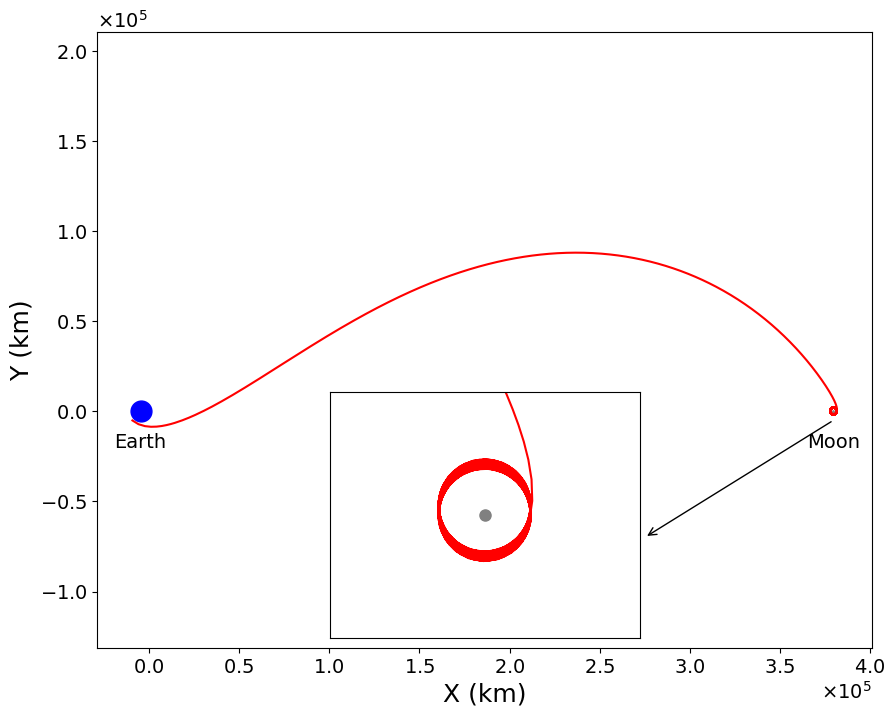
\includegraphics[width=\columnwidth]{figures/trajectory_rotating.png}
    \caption{Optimal $\Delta v_{total}$ bi-impulsive transfer from low Earth orbit to low lunar orbit as viewed from the Z axis in the rotating Earth-Moon frame.}
    \label{fig:trajectory}
\end{figure}

To assess the sensitivities in the optimal decision values, $N=400{,}000$ points were sampled randomly from uniform distributions over the final grid cell of the hierarchical grid search. The results are shown in Fig.~\ref{fig:MonteCarloSweep}.

The Jacobi integral was calculated in non-dimensional units at each time step of the integration to assess the convergence of the integration method. The deviation from the time-averaged value is plotted in Fig.~\ref{fig:JacobiIntegral}. The standard deviation was found to be $\sigma = 4.9 \times 10^{-12}$ confirming sufficent convergence.

\begin{figure}[h]
    \centering
    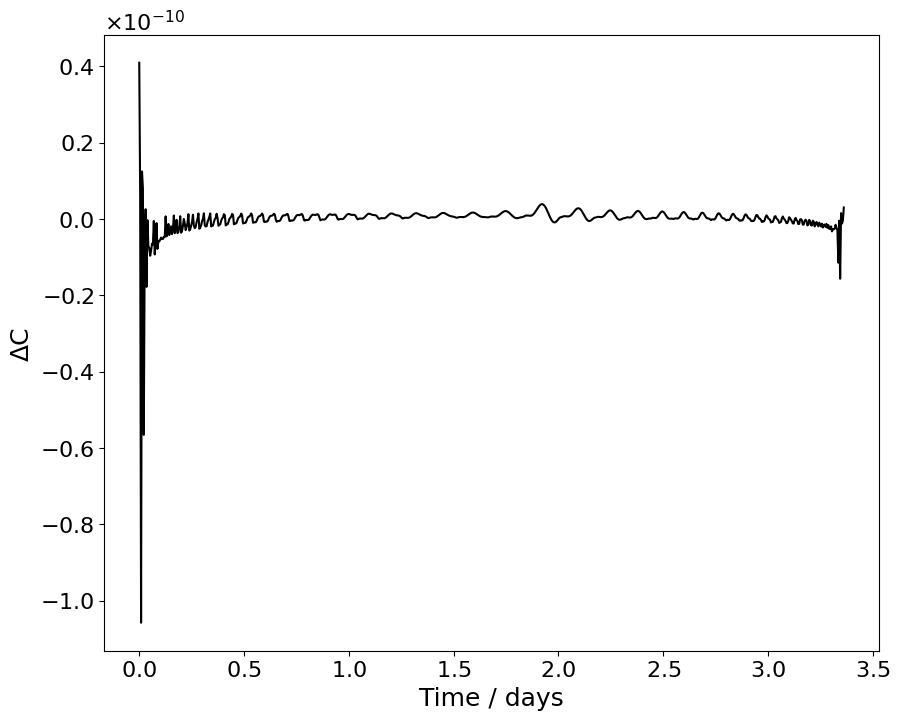
\includegraphics[width=\columnwidth]{figures/Jacobi Integral.png}
    \caption{Jacobi integral over time relative to the average value.}
    \label{fig:JacobiIntegral}
\end{figure}

\begin{figure*}[t]
    \centering
    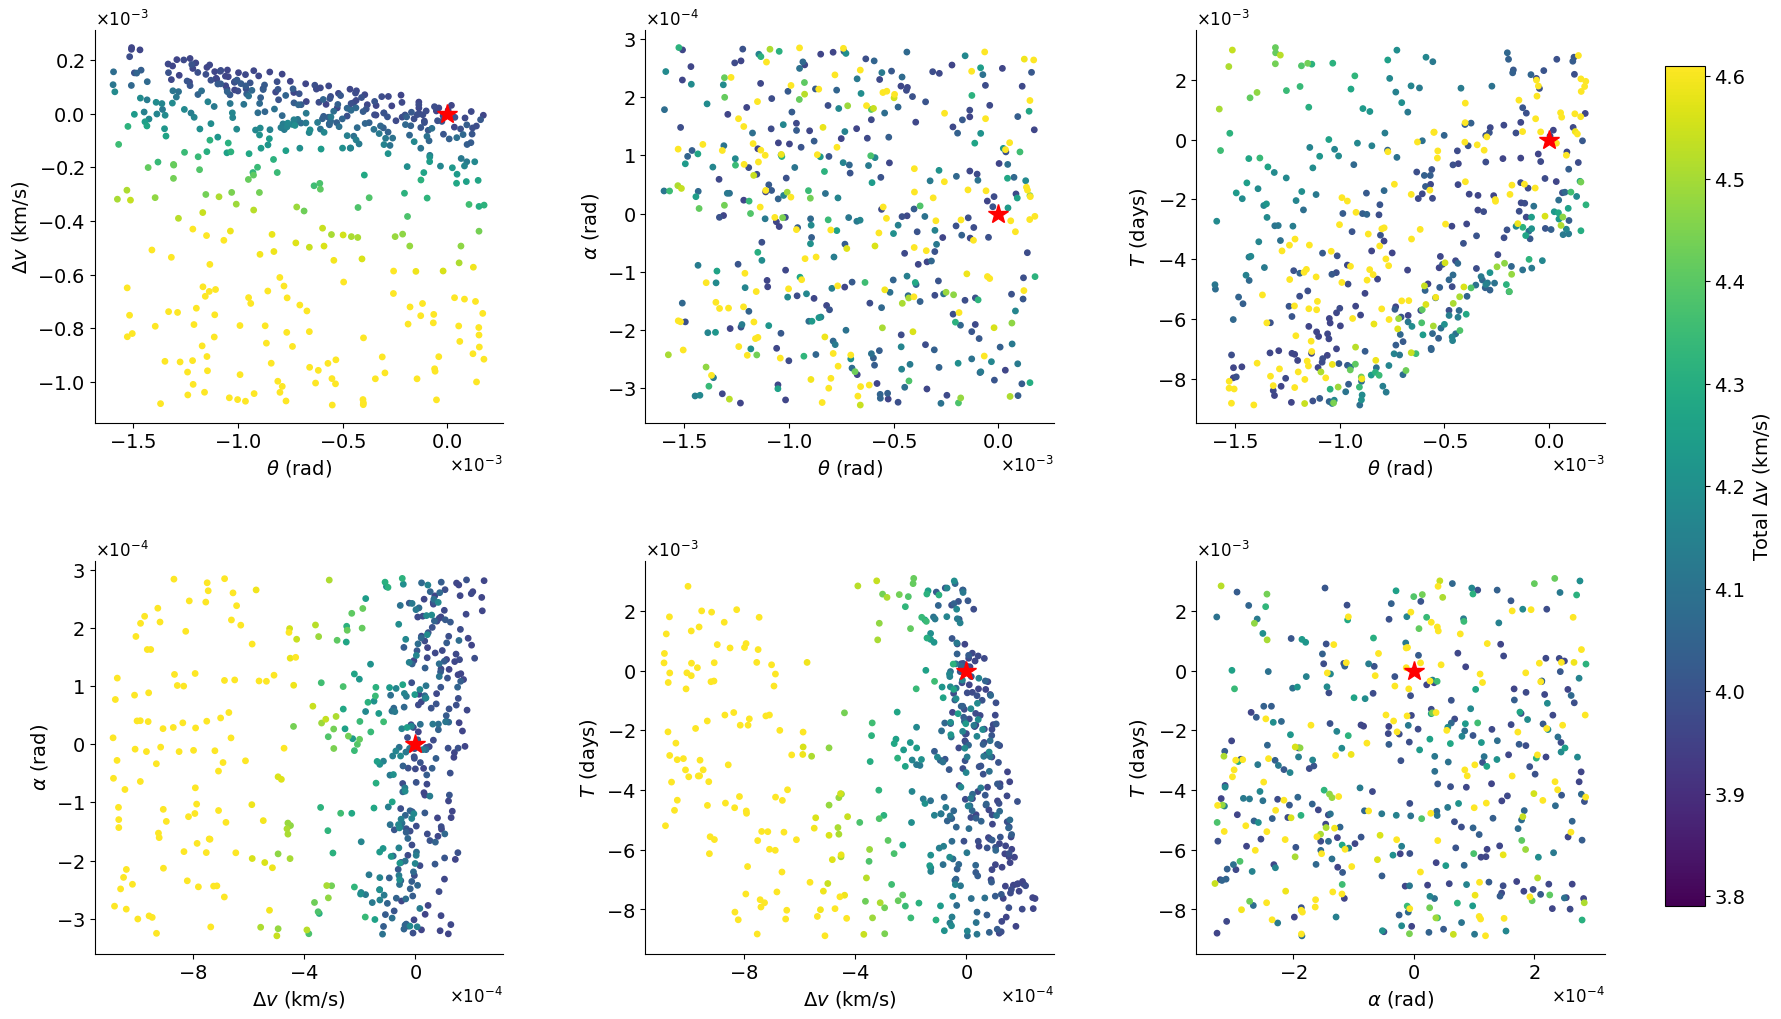
\includegraphics[width=\textwidth]{figures/MonteCarloSweep.png}
    \caption{2D slices of the 4D decision variable space for the Monte Carlo sensitivity analysis. The colour of the dots indicate the $\Delta v_{total}$ value White spaces indicate unfeasible regions (i.e regions where the constraint was not met). The optimal values of the decision variables are marked with red stars.}
    \label{fig:MonteCarloSweep}
\end{figure*}

\section{Discussion} 
\label{sec:Discussion}

The value obtained for the minimum total change in velocity for the manoeuvres required was $\Delta v_{total}=3.958~\mathrm{km/s}$. This value is 0.09\% larger than that obtained for a Hohmann transfer in the two body problem ($\Delta v_{total} = 3.954~\mathrm{km/s}$). Hence, according to the Rocket Equation (Eq.~\ref{Eq:RocketEquation}), the optimal trajectory found in this report does not save fuel compared to the Hohmann transfer.

As summarised by Topputo, finding solutions with significantly lower $\Delta v_{\mathrm{total}}$ (by $\sim 50~\mathrm{m/s}$) than the Hohmann transfer requires searching a much larger range of time of flight, $T$, up to two orders of magnitude greater than the bounds in Table~\ref{tab:bounds} \cite{topputo2013}. Topputo reports bi-impulsive solutions as low as $\Delta v_{\mathrm{total}} = 3.894~\mathrm{km/s}$ for $T \approx 255~\mathrm{days}$, representing a $\sim 1.5\%$ reduction over the Hohmann value. Larger times of flight allow the spacecraft to exploit lunar gravitational perturbation, the mechanism by which three body dynamics admit lower $\Delta v$ solutions. 

The proximity of the obtained value to the Hohmann transfer baseline suggests that the grid search converged to a local, rather than the global, optimum. The primary source of the discrepancy between the values is likely the unsuitability of the grid search to the inherent chaotic nature of the PCR3BP. The PCR3BP's phase space is multi-fractal at all levels, meaning there is no characteristic length scale below which it becomes smooth. This was shown by Trani in the general three body problem down to the scale of Planck length~\cite{trani2024}. Hence, for any grid with a finite number of points sampled, the global minimum can always lie between the sample points. This is a well established problem in spacecraft trajectory optimisation that can cause even the most sophisticated methods to fail ~\cite{izzo2007}.

The fractal nature of the decision variable space is shown in Fig.~\ref{fig:MonteCarloSweep}. Two distinct behaviours are observed due to the anisotropy of the objective function (Eq.~\ref{eq:opt_obj}) with respect to the decision variables. Firstly, as the objective function depends explicitly on $\Delta v_{1}$, the plots containing $\Delta v_{1}$ show clear gradients, with the optimal solution lying close to the border of infeasibility. Higher values of $\Delta v_{1}$ lead to lower values of $\Delta v_{total}$. This is because of the arrival geometry. Larger $\Delta v_{1}$ values arrive more tangential to the circular LLO orbit, reducing the $\Delta v_{2}$ insertion value, and consequently the overall $\Delta v_{total}$. Secondly, Eq.~\ref{eq:opt_obj} only depends on $\theta$, $\alpha$ and $T$ implicitly through $\Delta v_{2}$. Hence, the plots not containing $\Delta v_{1}$ show more random distributions as expected due to the fractal nature of the phase space.   

Another source of discrepancy is due to Algorithm~\ref{alg:hgs} being a greedy algorithm. At each level, the decision variables which best satisfy the constraint are chosen to be refined about and all other solutions at that level are permanently discarded. It is possible that due to narrow corridors of feasibility in the PCR3BP that the global optimum could be missed in these early levels and a local optimum is found instead. Furthermore, the fractal structure of the 4D decision variable space implies that fine-scale structure is uncorrelated with coarse-scale structure. To mitigate this, Algorithm~\ref{alg:hgs} could be extended to search the top $M$ results at each level. However, this would increase computational complexity by a factor of $M$. Algorithm~\ref{alg:hgs} has time complexity $\mathcal{O}(LN^{4}) $ and a current run time of $\sim 20~$ hours, with the suggested improvement it would become $\mathcal{O}(M LN^{4}) $ where L is the level of refinement and N is the number of grid points, as outlined in Section~\ref{sec:optimisation}. Due to the limited time to complete this project, this suggested improvement was not implemented.

A minor source of discrepancy between the $\Delta v_{total}$ value obtained in this report and the Hohmann transfer is the numerical integration error. DOP853 was the chosen integration method for this project. To help achieve sufficient convergence, the equations of motion \eqref{eq:EOM1} \eqref{eq:EOM2} were integrated in non-dimensional coordinates, making all the decision variables $\mathcal{O}(1)$. In Eq.~\ref{eq:sc}, when the decision variables are $\mathcal{O}(1)$, both $atol$ and $rtol$ are comparable, giving uniform error control across all variables. The convergence of the integration method was verified by plotting the Jacobi integral over time. As the Jacobi integral is a constant of motion, any deviation from the initial value is due to numerical errors. The Jacobi integral spikes to $1 \times 10^{-10}$ near the Earth and $1 \times 10^{-11}$ near the Moon. In these regions the gravitational potential varies as $1/r$, producing large and rapidly changing potential energy terms that the integrator must resolve over short timescales. The Jacobi integral is the difference between kinetic and potential energies. When both of these values are large but similar, the difference leads to a large floating point error. However, the standard deviation of the Jacobi integral was found to be $\sigma = 4.9 \times 10^{-12}$, which is similar to the accuracy of the integration method $atol = rtol = 1 \times 10^{-12}$. This indicates that sufficient convergence was achieved and the error due to numerical integration is negligible.

Grid searches cannot effectively explore the expanded decision variable space required to beat the Hohmann transfer, due to the time complexity and fractal structure of the PCR3BP phase space. Feasible solutions lie in narrow, fractally distributed corridors that no finite resolution grid is guaranteed to resolve. Increasing the integration time by two orders of magnitude means an exhaustive grid search would have a run time of $\sim 2000~\mathrm{hours}$. Further work could include using more sophisticated non-linear programming methods with a lower time complexity to search a larger decision variable space. For example, Sparse Nonlinear Optimizer (SNOPT) is a software package used by NASA in their General Mission Analysis Tool (GMAT)~\cite{gill2005, conway2010}. The optimal decision variables obtained by this investigation could be used as an initial guess and SNOPT could then be used to find the global optimum for a larger range of $T$.

\section{Conclusions}

This investigation aimed to find a bi-impulsive transfer trajectory in the PCR3BP from a Low Earth Orbit of altitude 167~km to a Low Lunar Orbit of altitude 100~km using less fuel than a Hohmann transfer. The problem was formulated as a non-linear programming problem and solved using a hierarchical grid search. The value obtained for the total change in velocity required was $\Delta v_{total} = 3.958~\mathrm{km/s}$ to a 5\% tolerance, which is 0.09\% higher than the Hohmann transfer value of $\Delta v_{total} = 3.954~\mathrm{km/s}$. The optimal trajectory found does not save fuel over the Hohmann transfer. For direct transfers at short times of flight, the lunar gravitational perturbation is insufficient to open lower cost pathways, and the two body Hohmann approximation remains adequate. 

Topputo has shown that significantly lower $\Delta v$ solutions exist at times of flight up to two orders of magnitude longer~\cite{topputo2013}, but the $\mathcal{O}(LN^{4})$ time complexity of the grid search prohibits exploration of this expanded region. Further work could employ more sophisticated non-linear programming methods such as SNOPT~\cite{gill2005}, using the solution obtained here as an initial guess to search a wider range of~$T$.

\section{Generative AI Statement}

In this report, Generative AI (Anthropic's Claude) was used to help with LaTeX formatting. Specifically in creating Figs. \ref{fig:cr3bp}, \ref{fig:Hohmann transfer}, \ref{fig:earth-moon-transfer} and Algorithm. \ref{alg:hgs}.

Microsoft's Copilot's autocomplete tab feature was used to help write the code.

\begin{acknowledgments}

The author would like to thank Dr. Scaringi for his excellent guidance and helpful support throughout this project.    

\end{acknowledgments}

\begin{thebibliography}{9}

\bibitem{ESA_ref_cornerstone}
European Space Agency, ``ESA Strategy for Science at the Moon.'' \url{https://exploration.esa.int/web/moon/-/61371-esa-strategy-for-science-at-the-moon}, (2019). Accessed \today.

\bibitem{nasa_artemis}
National Aeronautics and Space Administration,
``Artemis.''
\url{https://www.nasa.gov/humans-in-space/artemis/}, (2022).
Accessed \today.

\bibitem{jones2023}
H.W. Jones, ``Take Material to Space or Make It There?,''
in \textit{Proc. AIAA ASCEND Conference}, Las Vegas, NV, October 2023.
NASA Technical Reports Server, \url{https://ntrs.nasa.gov/citations/20230013555}.
Accessed \today.

\bibitem{nasa_rocket_equation}
NASA Glenn Research Center, ``Ideal Rocket Equation.''
\url{https://www1.grc.nasa.gov/beginners-guide-to-aeronautics/ideal-rocket-equation/}.
Accessed \today.

\bibitem{tsiolkovsky1903}
K.E. Tsiolkovsky, ``Investigation of Cosmic Space by Means of Reaction Devices,''
\textit{Nauchnoe Obozrenie} \textbf{5}, 45--75 (1903).

\bibitem{Hohmann1925}
W. Hohmann, \textit{Die Erreichbarkeit der Himmelsk\"{o}rper}
(Oldenbourg, Munich, 1925);
NASA Technical Translation F-44 (1960).

\bibitem{Riche1969}
L.J. Riche, G.M. Colton, and T.A. Guillory,
\textit{Flight Plan Apollo 11}
(NASA, Houston, Texas, 1969).

\bibitem{Belbruno1993}
E.A. Belbruno and J.K. Miller,
``Sun-Perturbed Earth-to-Moon Transfers with Ballistic Capture,''
\textit{J. Guid. Control Dyn.} \textbf{16}, 770--775 (1993).
doi: 10.2514/3.21079.

\bibitem{roncoli2010}
R.B. Roncoli and K.K. Fujii, ``Mission Design Overview for the Gravity Recovery
and Interior Laboratory ({GRAIL}) Mission,''
in \textit{Proc. AIAA/AAS Astrodynamics Specialist Conference},
Toronto, Canada, August 2010, AIAA 2010-8383.

\bibitem{Sweetser1991}
T.H. Sweetser,
``An Estimate of the Global Minimum $\Delta v$ Needed for Earth--Moon Transfer,''
\textit{Adv. Astronaut. Sci.} \textbf{75}, 111--120 (1991).

\bibitem{topputo2013}
F. Topputo, ``On Optimal Two-Impulse Earth--Moon Transfers in a Four-Body Model,''
\textit{Celest. Mech. Dyn. Astron.} \textbf{117}, 279--313 (2013).
doi: 10.1007/s10569-013-9513-8.

\bibitem{Qi_Xu_2016}
Y. Qi and S. Xu, ``Minimum $\Delta v$ for the Transfer to Permanent Lunar Orbits
with Hyperbolic Approach,''
\textit{Acta Astronaut.} \textbf{119}, 183--195 (2016).
doi: 10.1016/j.actaastro.2015.11.016.

\bibitem{hairer1993}
E. Hairer, S.P. N{\o}rsett, and G. Wanner,
\textit{Solving Ordinary Differential Equations I: Nonstiff Problems}, 2nd ed.
(Springer-Verlag, Berlin, 1993).

\bibitem{virtanen2020}
P. Virtanen \textit{et al.}, ``SciPy 1.0: Fundamental Algorithms for Scientific
Computing in Python,''
\textit{Nat. Methods} \textbf{17}, 261--272 (2020).
doi: 10.1038/s41592-019-0686-2.

\bibitem{ESA_ref_5}
SRE-PA \& D-TEC staff, ``Margin Philosophy for Science Assessment Studies,''
ESA Technical Note, SRE-PA/2011.097/, Issue 1, Rev. 3 (2012).
\url{https://sci.esa.int/documents/34375/36249/1567260131067-Margin\_philosophy\_for\_science\_assessment\_studies\_1.3.pdf}.
Accessed \today.

\bibitem{trani2024}
A.A. Trani \textit{et al.}, ``Isles of Regularity in a Sea of Chaos amid the
Gravitational Three-Body Problem,''
\textit{Astron. Astrophys.} \textbf{689}, A24 (2024).
doi: 10.1051/0004-6361/202449862.

\bibitem{izzo2007}
D. Izzo \textit{et al.}, ``Search Space Pruning and Global Optimisation of Multiple
Gravity Assist Spacecraft Trajectories,''
\textit{J. Glob. Optim.} \textbf{38}, 283--296 (2007).
doi: 10.1007/s10898-006-9106-0.

\bibitem{gill2005}
P.E. Gill, W. Murray, and M.A. Saunders, ``SNOPT: An SQP Algorithm for
Large-Scale Constrained Optimization,''
\textit{SIAM Rev.} \textbf{47}, 99--131 (2005).
doi: 10.1137/S0036144504446096.

\bibitem{conway2010}
D.J. Conway and S.P. Hughes, ``The General Mission Analysis Tool ({GMAT}):
Current Features and Adding Custom Functionality,''
in \textit{Proc. International Conference on Astrodynamics Tools and Techniques (ICATT)},
Madrid, Spain, May 2010, NASA/TM-20180000083.

\end{thebibliography}

\newpage

\clearpage

\section*{Error Appendix}

Unlike experimental investigations, computational studies are subject to numerical and statistical errors arising from algorithmic limitations. 

In this project, the "errors" were estimated using Monte Carlo sampling. $N=400{,}000$ points were uniformly sampled within the final grid cell of the hierarchical search. The resulting $\Delta v_{total}$ was recorded for each combination of decision variables. The 4D decision variable space was then filtered to only look at points with a $\Delta v_{total}$ within 5\% of the optimal value. This tolerance was chosen as it is the current industry standard for the European Space Agency \cite{ESA_ref_5}. 

2D projections of the 4D decision variable space are plotted below in Figs. \ref{fig:MonteCarloSweep1}-\ref{fig:MonteCarloSweep3}. Only the three projections on which the extremal bounds of the decision variables are largest are shown; the remaining three projections have narrower ranges and are omitted for brevity.

\begin{figure}[h!]
    \centering
    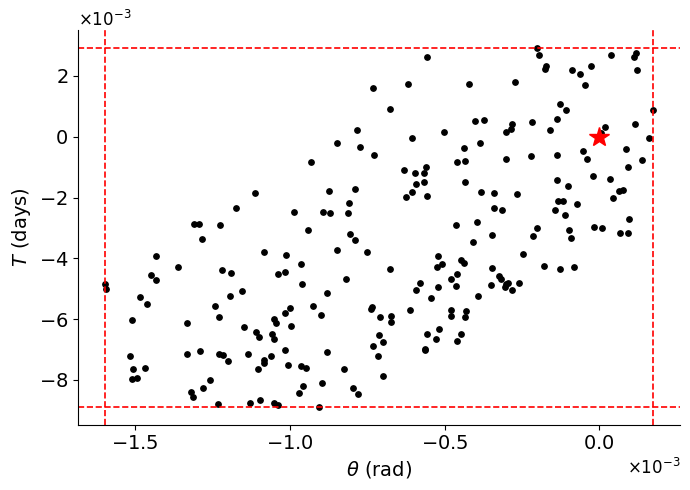
\includegraphics[width=0.48\textwidth]{figures/MonteCarloSweep1.png}
    \caption{$T - \theta$ slice of the 4D decision variable space. Black dots indicate a viable solution with a $\Delta v_{total}$ within 5\% of the optimal value. The optimal values are marked with stars. The red borders show the minimum and maximum for each of the 4 decision variables.}
    \label{fig:MonteCarloSweep1}
\end{figure}

\begin{figure}[h!]
    \centering
    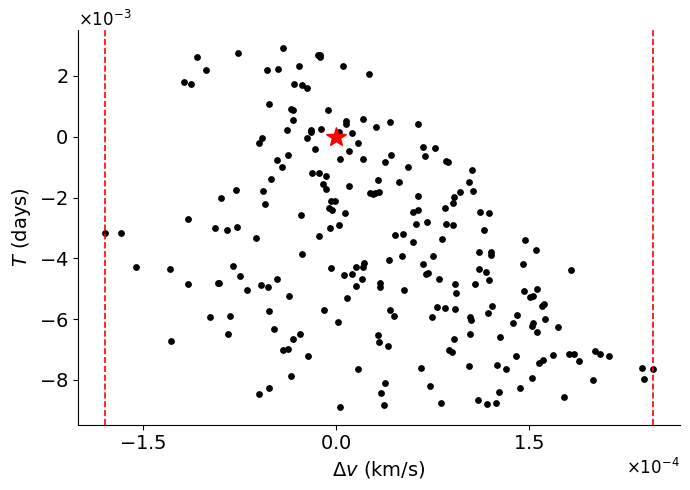
\includegraphics[width=0.48\textwidth]{figures/MonteCarloSweep2.png}
    \caption{$T - \Delta v$ slice of the 4D decision variable space. Black dots indicate a viable solution with a $\Delta v_{total}$ within 5\% of the optimal value. The optimal values are marked with stars. The red borders show the minimum and maximum.}
    \label{fig:MonteCarloSweep2}
\end{figure}

\begin{figure}[h!]
    \centering
    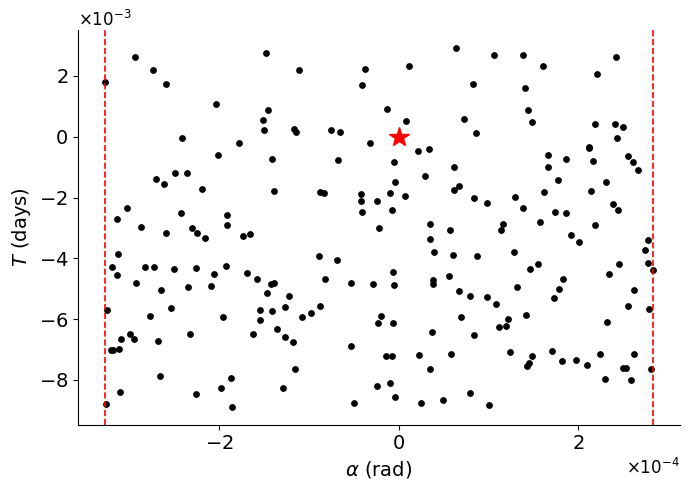
\includegraphics[width=0.48\textwidth]{figures/MonteCarloSweep3.png}
    \caption{$T - \alpha$ slice of the 4D decision variable space. Black dots indicate a viable solution with a $\Delta v_{total}$ within 5\% of the optimal value. The optimal values are marked with stars. The red borders show the minimum and maximum for each of the 4 decision variables.}
    \label{fig:MonteCarloSweep3}
\end{figure}
\clearpage

\onecolumngrid %Puts Summary into single column

\section*{Scientific Summary for a General Audience}

\begin{quote}
\textit{``Earth is the cradle of humanity, but one cannot live in a cradle forever.''}\\
\hfill --- Konstantin Tsiolkovsky
\end{quote}

Reaching the Moon is no longer a question of possibility; it is a question of cost. SpaceX's Falcon 9 rocket, one of the most advanced rockets ever made, costs $\$2{,}940$ to send a single kilogram of payload into orbit. At this price, even modest spaceflight missions cost hundreds of millions of dollars. The Rocket Equation says that exponentially more fuel is required to accelerate more payload mass, meaning a typical rocket is 90\% fuel by mass. Reducing the amount of fuel, therefore has an outsized effect on bringing down the mission cost.

The aim of this investigation was to find the minimum fuel transfer trajectory between low Earth orbit and low lunar orbit (the usual start and end points for transfers to the moon). A bi-impulsive transfer uses exactly two engine burns: the first accelerates the spacecraft out of Earth orbit, and the second slows it into lunar orbit. By systematically varying the departure position, departure velocity, and the timing of the second burn across thousands of simulated trajectories, the combination requiring the least total fuel is identified.

\end{document}